\documentclass{article} %document style and layout
\usepackage{enumitem} %list of elements
\usepackage{imakeidx}
\usepackage{hyperref}
\usepackage{xcolor}
\usepackage{graphicx}
\usepackage{subcaption}
% \usepackage[utf8]{inputenc}
% \usepackage[T1]{fontenc}
\usepackage{listings} %package to import code
\lstdefinestyle{mystyle}{
    backgroundcolor=\color{backcolour},   
    commentstyle=\color{code_green},
    keywordstyle=\color{url_blue},
    stringstyle=\color{orange},
    basicstyle=\ttfamily\footnotesize,
    breakatwhitespace=false,         
    breaklines=true,                 
    captionpos=b,                    
    keepspaces=true,                 
    numbers=left,                    
    numbersep=5pt,                  
    showspaces=false,                
    showstringspaces=false,
    showtabs=false,                  
    tabsize=2
}
\lstset{style=mystyle}

\usepackage{titling}
\renewcommand\maketitlehooka{\null\mbox{}\vfill}
\renewcommand\maketitlehookd{\vfill\null}

%-------Titlepage information------------------------------------------
\title{\textbf{\huge{Wireless internet - WiFi traffic classification.}}}
\author{Luca Ferraro (10748116), Fabio Losavio (10567493) \\ 
\textcolor{url_blue}{\url{https://github.com/LucaFerraro/Wireless_internet_project}}}
\date{A.Y. 2019/2020}
%----------------------------------------------------------------------

\begin{document}
\definecolor{url_blue}{rgb}{0,0.427,0.639} %rgb: 0, 109, 163 
\definecolor{backcolour}{rgb}{0.95,0.95,0.92}
\definecolor{code_green}{RGB}{11,102,35}

\begin{titlingpage}
    \maketitle
\end{titlingpage}

\newpage{}

\tableofcontents
\listoffigures
\lstlistoflistings
\newpage{}

%------------------------------------------------------------------------------------------------------------------------------------------------
\clearpage
\section{Introduction}
\label{sect:introduction}
The aim of this project is using the protocol analyzer \textit{Wireshark} for classifying traffic at \textit{MAC} layer.\\ 
To reach this goal, we used \textit{Wireshark} in \textit{monitor\ mode}: in this mode, the \textit{WiFi} module of our PC
intercepts all the traffic in range that is transiting via \textit{WiFi}.\\ 
This is a limitation for our project in the sense that at \textit{MAC} layer it's possible to check whether a frame is transporting data, but it's 
not possible to distinguish the application that has generated the data carried in the payload of the frame. Therefore, our 
analysis only provides a quantitative estimation of the traffic of data transported over \textit{WiFi}. The reason why we have 
used this solution even if we were aware of this limitation is that working in monitor mode is the only solution we had
to sniff traffic that was not meant only for the computer that was performing the capure.\\

\subsection{{Our analysis.}}
    In this project, what we have done is looking at the \textit{data} and \textit{QoS data} frames captured by our computers and
    try to understand what those packets are meant to in terms of type of application that has generated them. As specified, this 
    can only be a deduction: we can't be sure of the application that has generated a packet at \textit{MAC} layer.\\ 
    To do this we have scanned many sample captures and for each one of them:
    \begin{enumerate}
        \item Found all the \textit{MAC} addresses that have generated/received at least one \textit{data/QoS\ data} frame.
        \item Associated to all the \textit{MAC} addresses we have revealed:
        \begin{itemize}
            \item The number of transmitted/received bytes.
            \item The number of transmitted/received packets.
            \item The average uplink/downlink rate.
        \end{itemize}
        \item Found the vendor associated with the \textit{MAC} address.
    \end{enumerate}
    In order to analyze the captured traffic and try to understand the type of application a user (so a \textit{MAC}) was using,
    we have plotted: 
    \begin{itemize}
        \item A pair of histograms (one for the bytes, one for the number of packets) in which there is a bar for each
                \textit{MAC} address that have generated/received at least a certain amount of packets (better description of
                this later on).
        \item A graph for the cumulative uplink/downlink traffic (considering then all the bytes generated/received by all the 
                revealed \textit{MACs}).
        \item A graph for the discrete traffic in uplink/downlink, that is the total amount of bytes exchanged by all the revealed
                \textit{MACs} in a fixed time interval (customizable in the program).
    \end{itemize}


%------------------------------------------------------------------------------------------------------------------------------------------------
\clearpage
\section{Project description}
\label{sect:project}
\subsection{Program setup}
To launch and use the program, first some pre-requisites have to be meet:
\begin{itemize}
    \item install pyshark library in order to analyze the capture file 
    \item install numpy library to perform some numerical analysis
    \item install matplotlib library to visualize plots
\end{itemize}
The program can run in 3 different modes selected by adding an attribute to the standard 
python call, using the command \texttt{python Traffic\_analyzer.py -file "PATH TO A FILE"} 
the program will scan the file provided after the \textit{-file} parameter. In this mode the program
will open the selected capture (in a .pcap/.pcapng format) and start scanning all the packets in 
order to obtain some information. 

The second mode is the live capturing mode in which, using the command \texttt{sudo python
Traffic\_analyzer.py -live "INTERFACE" "DURATION"} the program will first start a 
capture on the given interface,that has to be enabled to work in monitor mode, for a given 
amount of time provided with the "DURATION" attribute, will save this capture and will work
on it. With this mode administrator privileges are required to allow tshark to start the 
capture in monitor mode.  

The last mode is a default mode, launched using the command \texttt{python Traffic\_analyzer.py},
which will perform the analysis on a default capture inserted in the code. This mode is mostly 
used as a debug tool but can also be useful to understand how the output will look like.

\subsection{Program structure}
To obtain information from a capture, the code will run a for loop on all the packets in the 
capture file and will analyze only those which can be useful for our purpose. To select the 
useful the following filter is used:

\begin{lstlisting}[language=Python, caption=Packet filter]
    (int(packet.wlan.fc_type) == 2) and 
    ((int(packet.wlan.fc_subtype) >= 0 and 
        int(packet.wlan.fc_subtype) <= 3)) or
    (int(packet.wlan.fc_subtype) >= 8 and 
    int(packet.wlan.fc_subtype) <= 11)
\end{lstlisting}

it will select all the \textbf{data} frames (wlan.fc\_type == 2) and among those it will 
select the ones actually containing data or QoS data excluding null packets or ACKs. From 
those packets it will extract the destination address and will add it to a dictionary. 


%------------------------------------------------------------------------------------------------------------------------------------------------
\clearpage
\section{Examples}
\label{sect:project}
% Descrivere cosa c'è di interessante nella cattura evidenziando i MAC che conosciamo, quelli che 
% fanno cose che abbiamo capito (ad esempio i sonos oppure i dispositivi che usano zoom) e inserire
% le immagini come contorno

<<<<<<< HEAD
To test our program we did some captures in different moments of the day to see what we are able to 
understand from it.
\subsection{Sonos speakers interconnected via WiFi}
=======
\subsection{Sonos capture.}
>>>>>>> 370de4e35883f001c1c6d3fcf0493189a25769a1
%Fabio
 A capture that brought something interesting to our attention is the \texttt{Filtered
\_capture\_SONOS\_WEDNESDAY\_MILAN.pcapng} done in Milan on a wednesday morning. Thanks to the vendor 
classification we spotted a four MAC addresses related to \textbf{Sonos} devices, a vendor famous for
wireless home sound systems in which multiple speakers are interconnected using WiFi. In this capture 
we found four different devices which produced most of the traffic, the MAC addresses of the Sonos 
devices are:
\begin{itemize}
    \item 00:0e:58:c2:48:5f
    \item 00:0e:58:c2:48:05
    \item 00:0e:58:67:a3:e9
    \item 00:0e:58:f4:7a:83
\end{itemize}
As we can see in Figure \ref{fig:Sonos_traffic}, there are a lot of traffic spikes mainly due to the
communication between those speakers. The highest peak is the combination of the communication between
the Sonos devices and other communication flows.
\begin{figure}[h]
    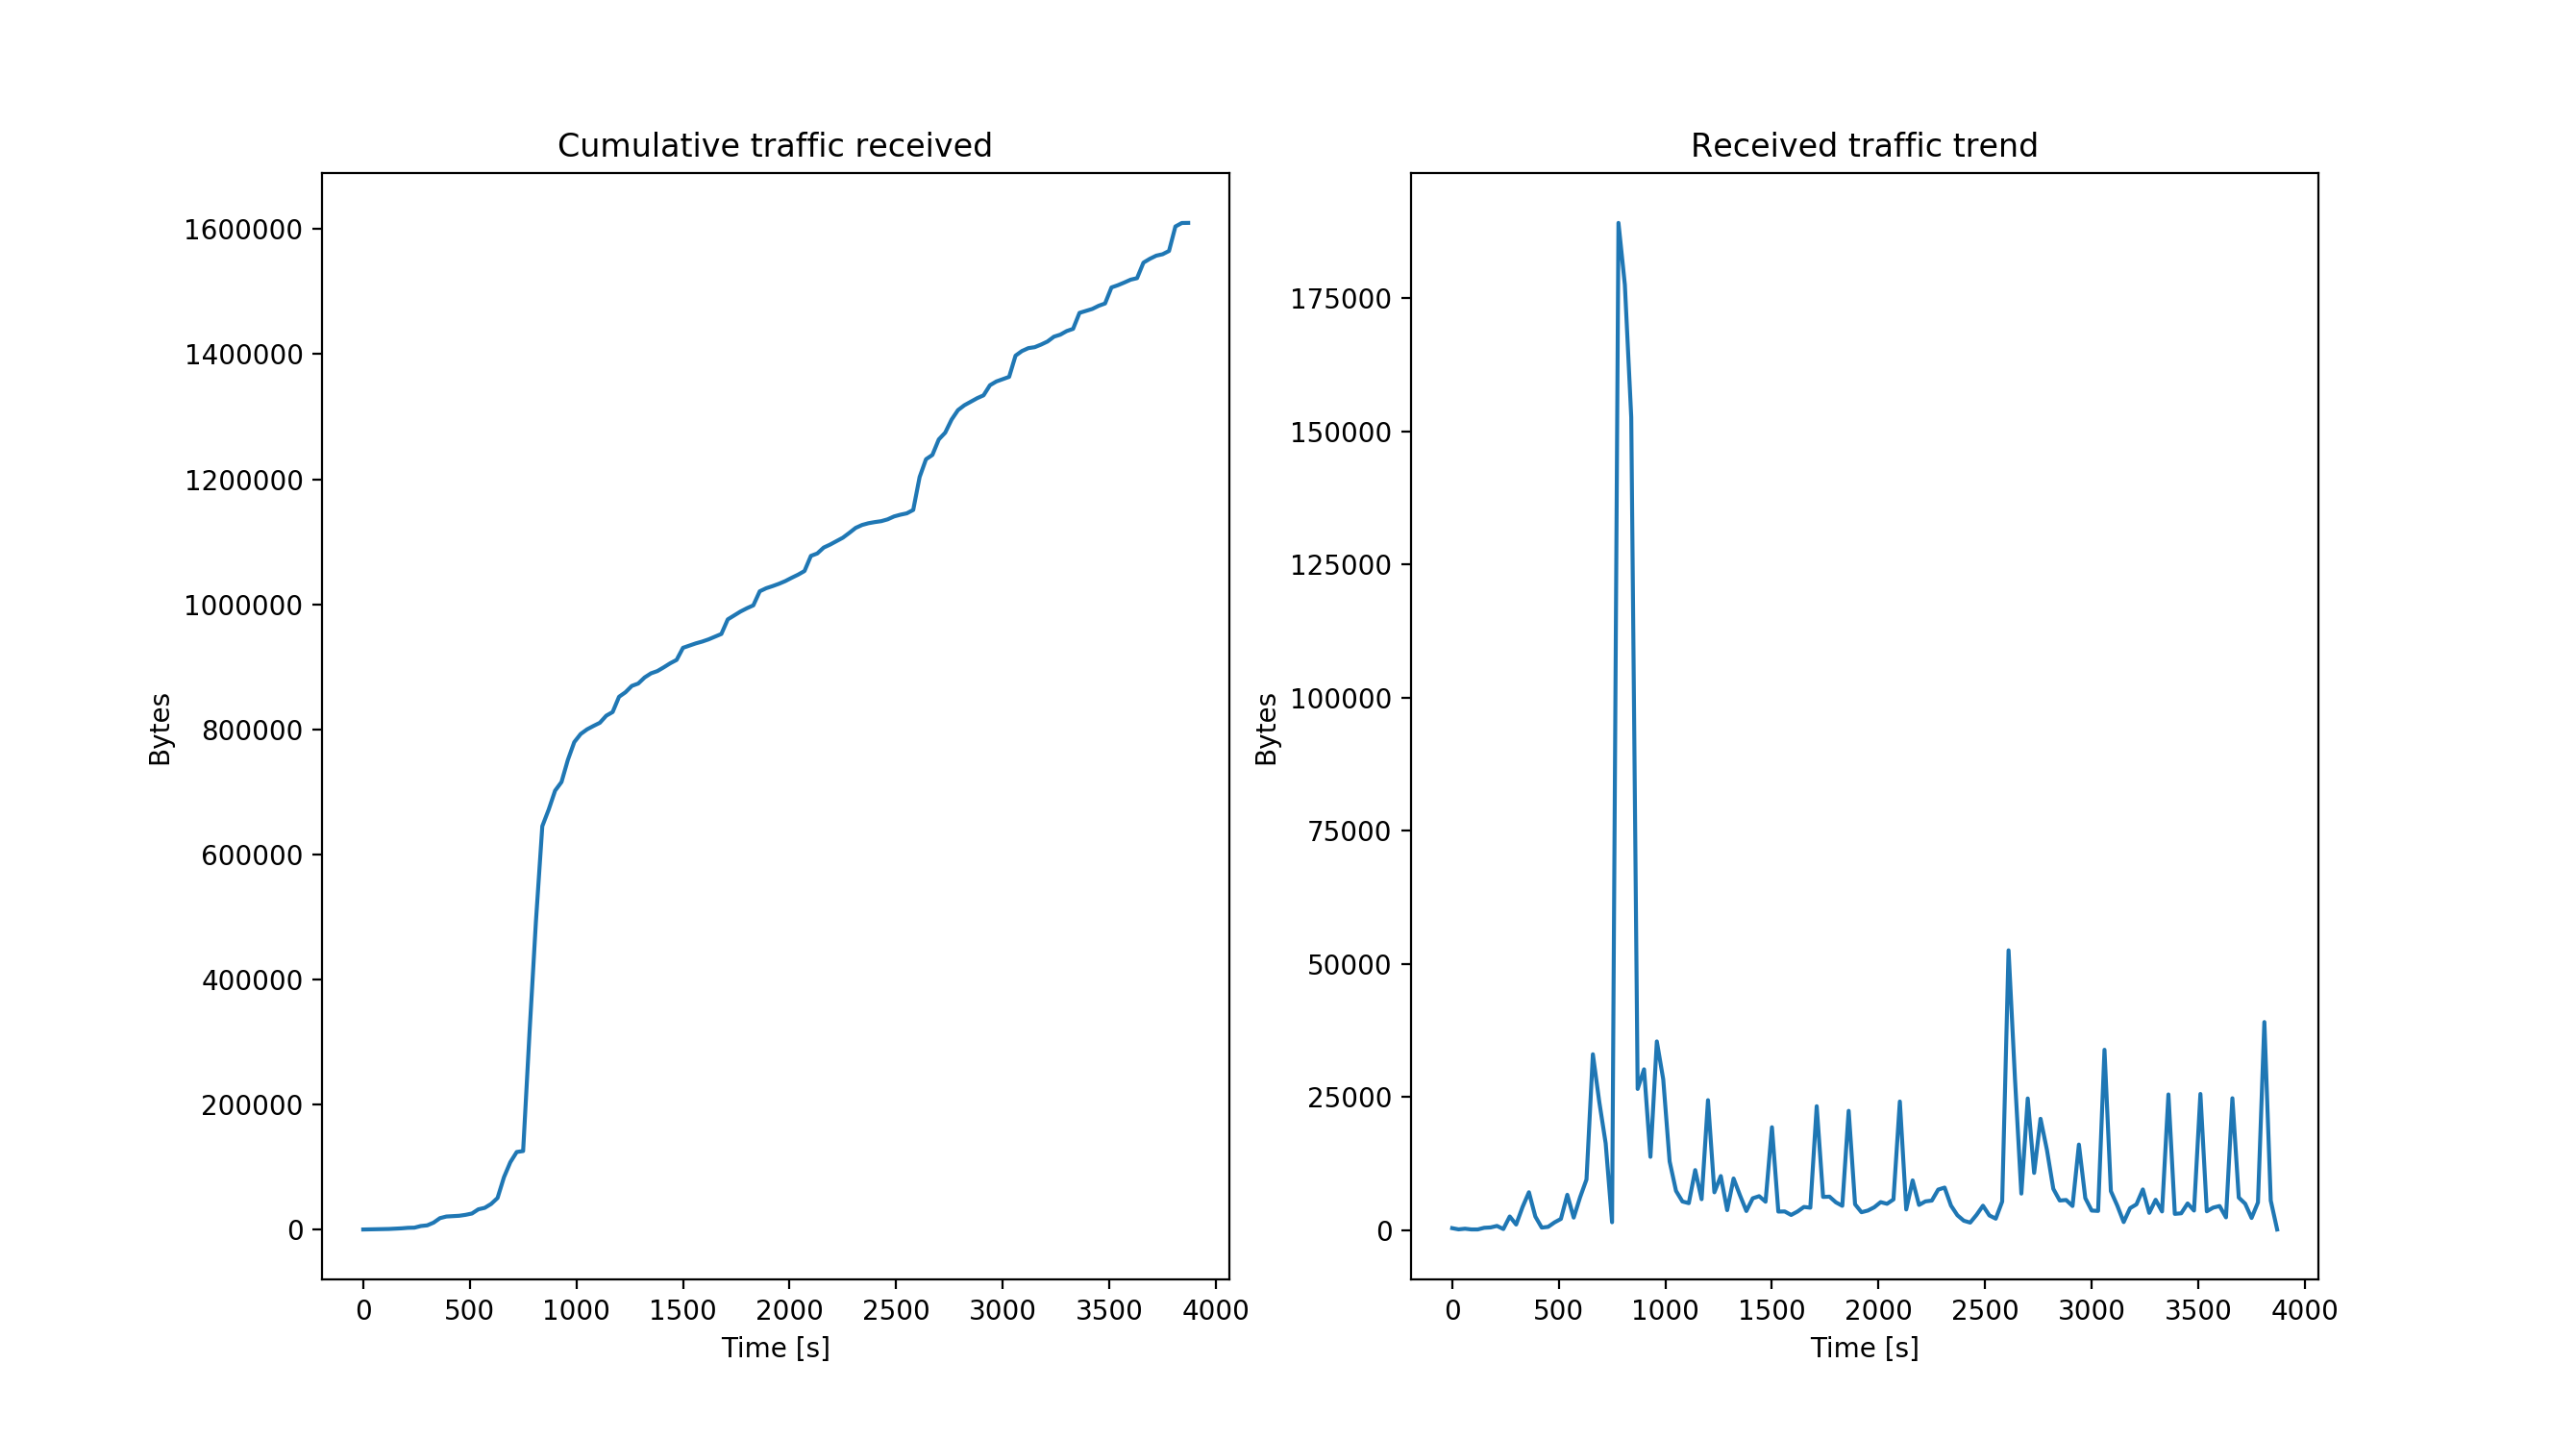
\includegraphics[width=\textwidth]{Graphs/SONOS_cum_in_traffic.png}
    \caption{Sonos input traffic graphs}
    \label{fig:Sonos_traffic}
\end{figure}
\\
To further show how many packets the Sonos devices exchanged we can see that three out of the four
devices are at the top spots of the following graph.
\begin{figure}[h]
    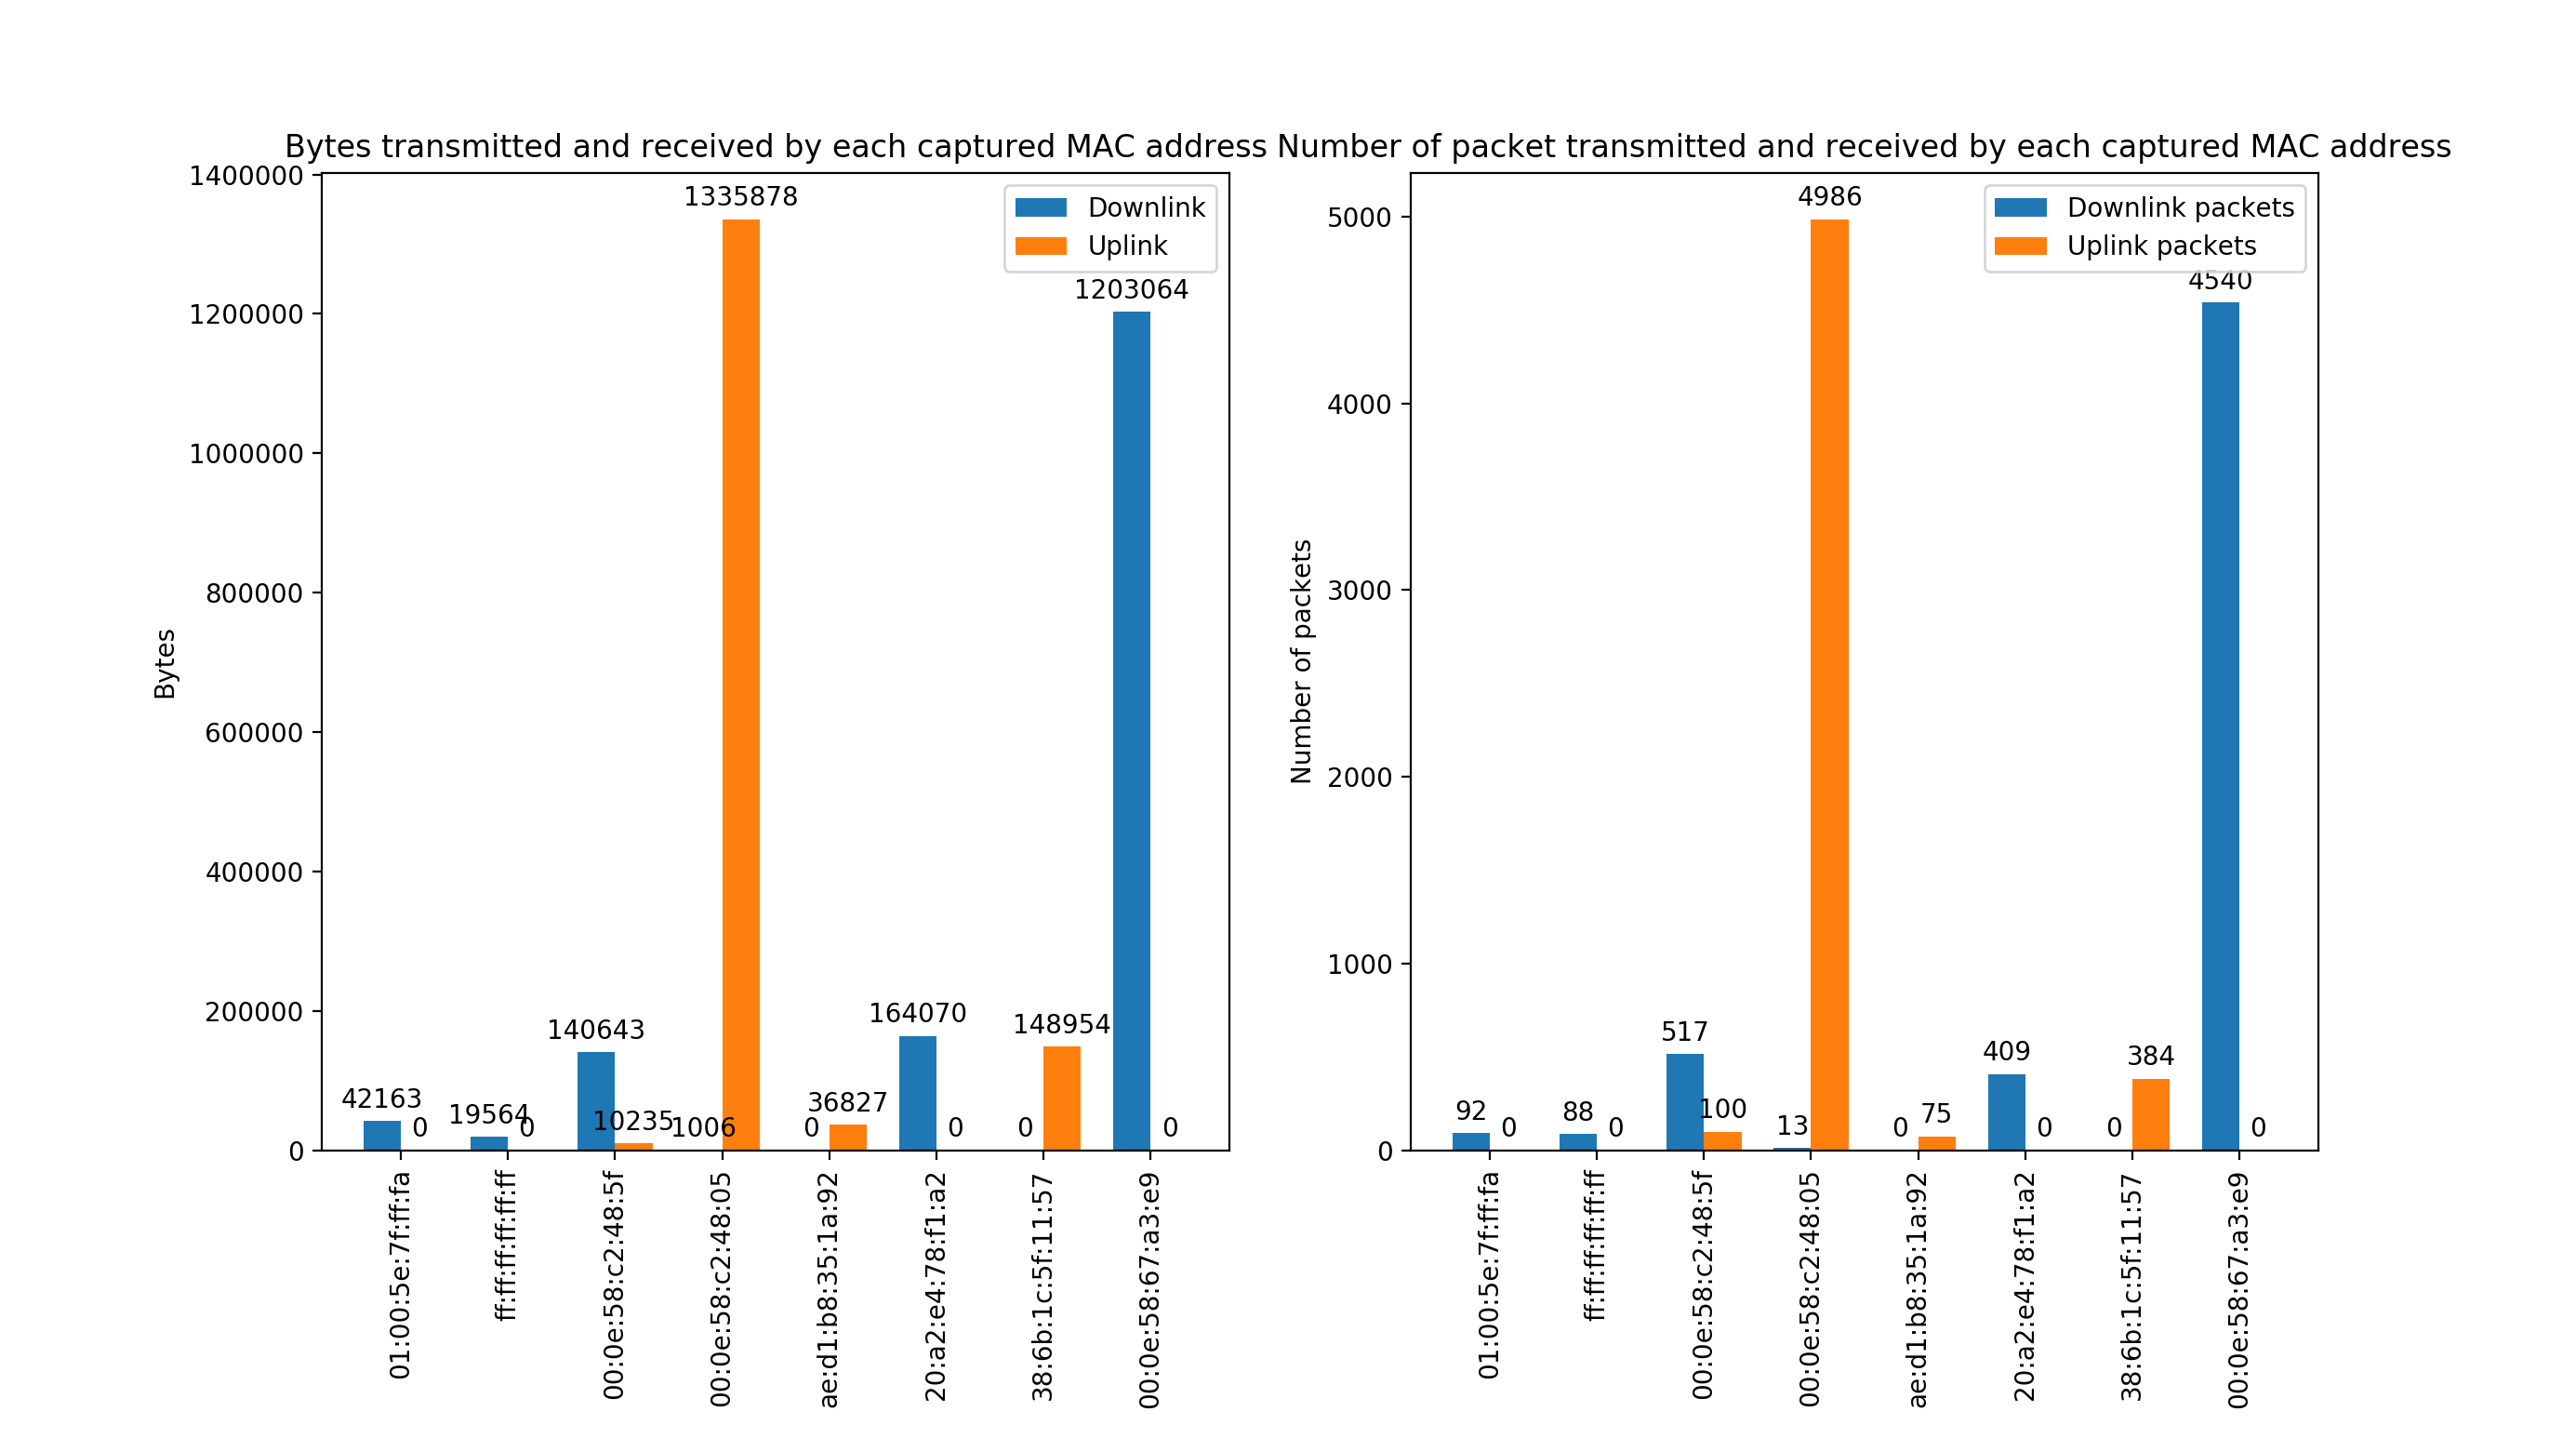
\includegraphics[width=\textwidth]{Graphs/SONOS_bytes_packets.png}
    \caption{Sonos packets exchanged}
    \label{fig:Sonos_packets}
\end{figure}

<<<<<<< HEAD

 
\subsection{ZOOM}
=======
\subsection{Zoom captures.}
>>>>>>> 370de4e35883f001c1c6d3fcf0493189a25769a1
%Fabio

\subsection{Multimedia internet capture.}
In this paragraph, we analyze the results obtained with a capture performed during a lecture of
multimedia internet. \\ 
The lecture has been followed using \textit{Microsoft\ Teams}: the professor was presenting the
topic sharing its screen and all the students were following him with camera and microphone inactive.\\
In the Figure \ref{Multimedia internet lecture: data and packets exchanged.}, we can see on the
left the graphs reporting the number of bytes transmitted and received by some of the \textit{MACs}
we have revealed and on the right the number of transmitted and received by the same \textit{MACs}.\\
As we can see, there are some \textit{MACs} that are exchanging much more traffic than others:

\begin{itemize}
    \item \textbf{88:ae:07:3d:8a:30}: this is the device (an \textit{iPad\ Pro}) from which the lecture 
            was being attended. Even if the capture lasted only 5 minutes, we can see that this 
            device has received a lot of bytes (about 42.660 MB): this is of course due to the fact
            that the device was using a video-conferencing application.\\ 
            If we consider the number of packets received by this \textit{MAC}, we can compute the 
            average length of the packets during the 5 minutes of the capture:

            \begin{equation}
                \textit{Average packet length} = \textit{Number of bytes} / \textit{Number of packets} = 594 Bytes
            \end{equation}

    \item \textbf{20:b0:01:22:22:66}: this is the access point of the home were the lecture was being
            attended. Indeed, we can see that the access point has sent a lot of bytes and packets: 
            most of them were probably destined to the \textit{iPad\ Pro} that was being used to
            follow the lecture, since that device was connected to this access point while attending 
            the class. 
\end{itemize}

Among the other \textit{MAC} addresses present in the graph but that have exchanged only a few 
packets in compared with the 2 ones mentioned above, we recognize only \textbf{dc:a9:04:91:42:b9}: 
it's a \textit{MacBook Pro} in the same home. During the 5 minutes of the capture, this device was 
being used for smart-working purposes.s

\begin{figure}[h!]
    \centering
    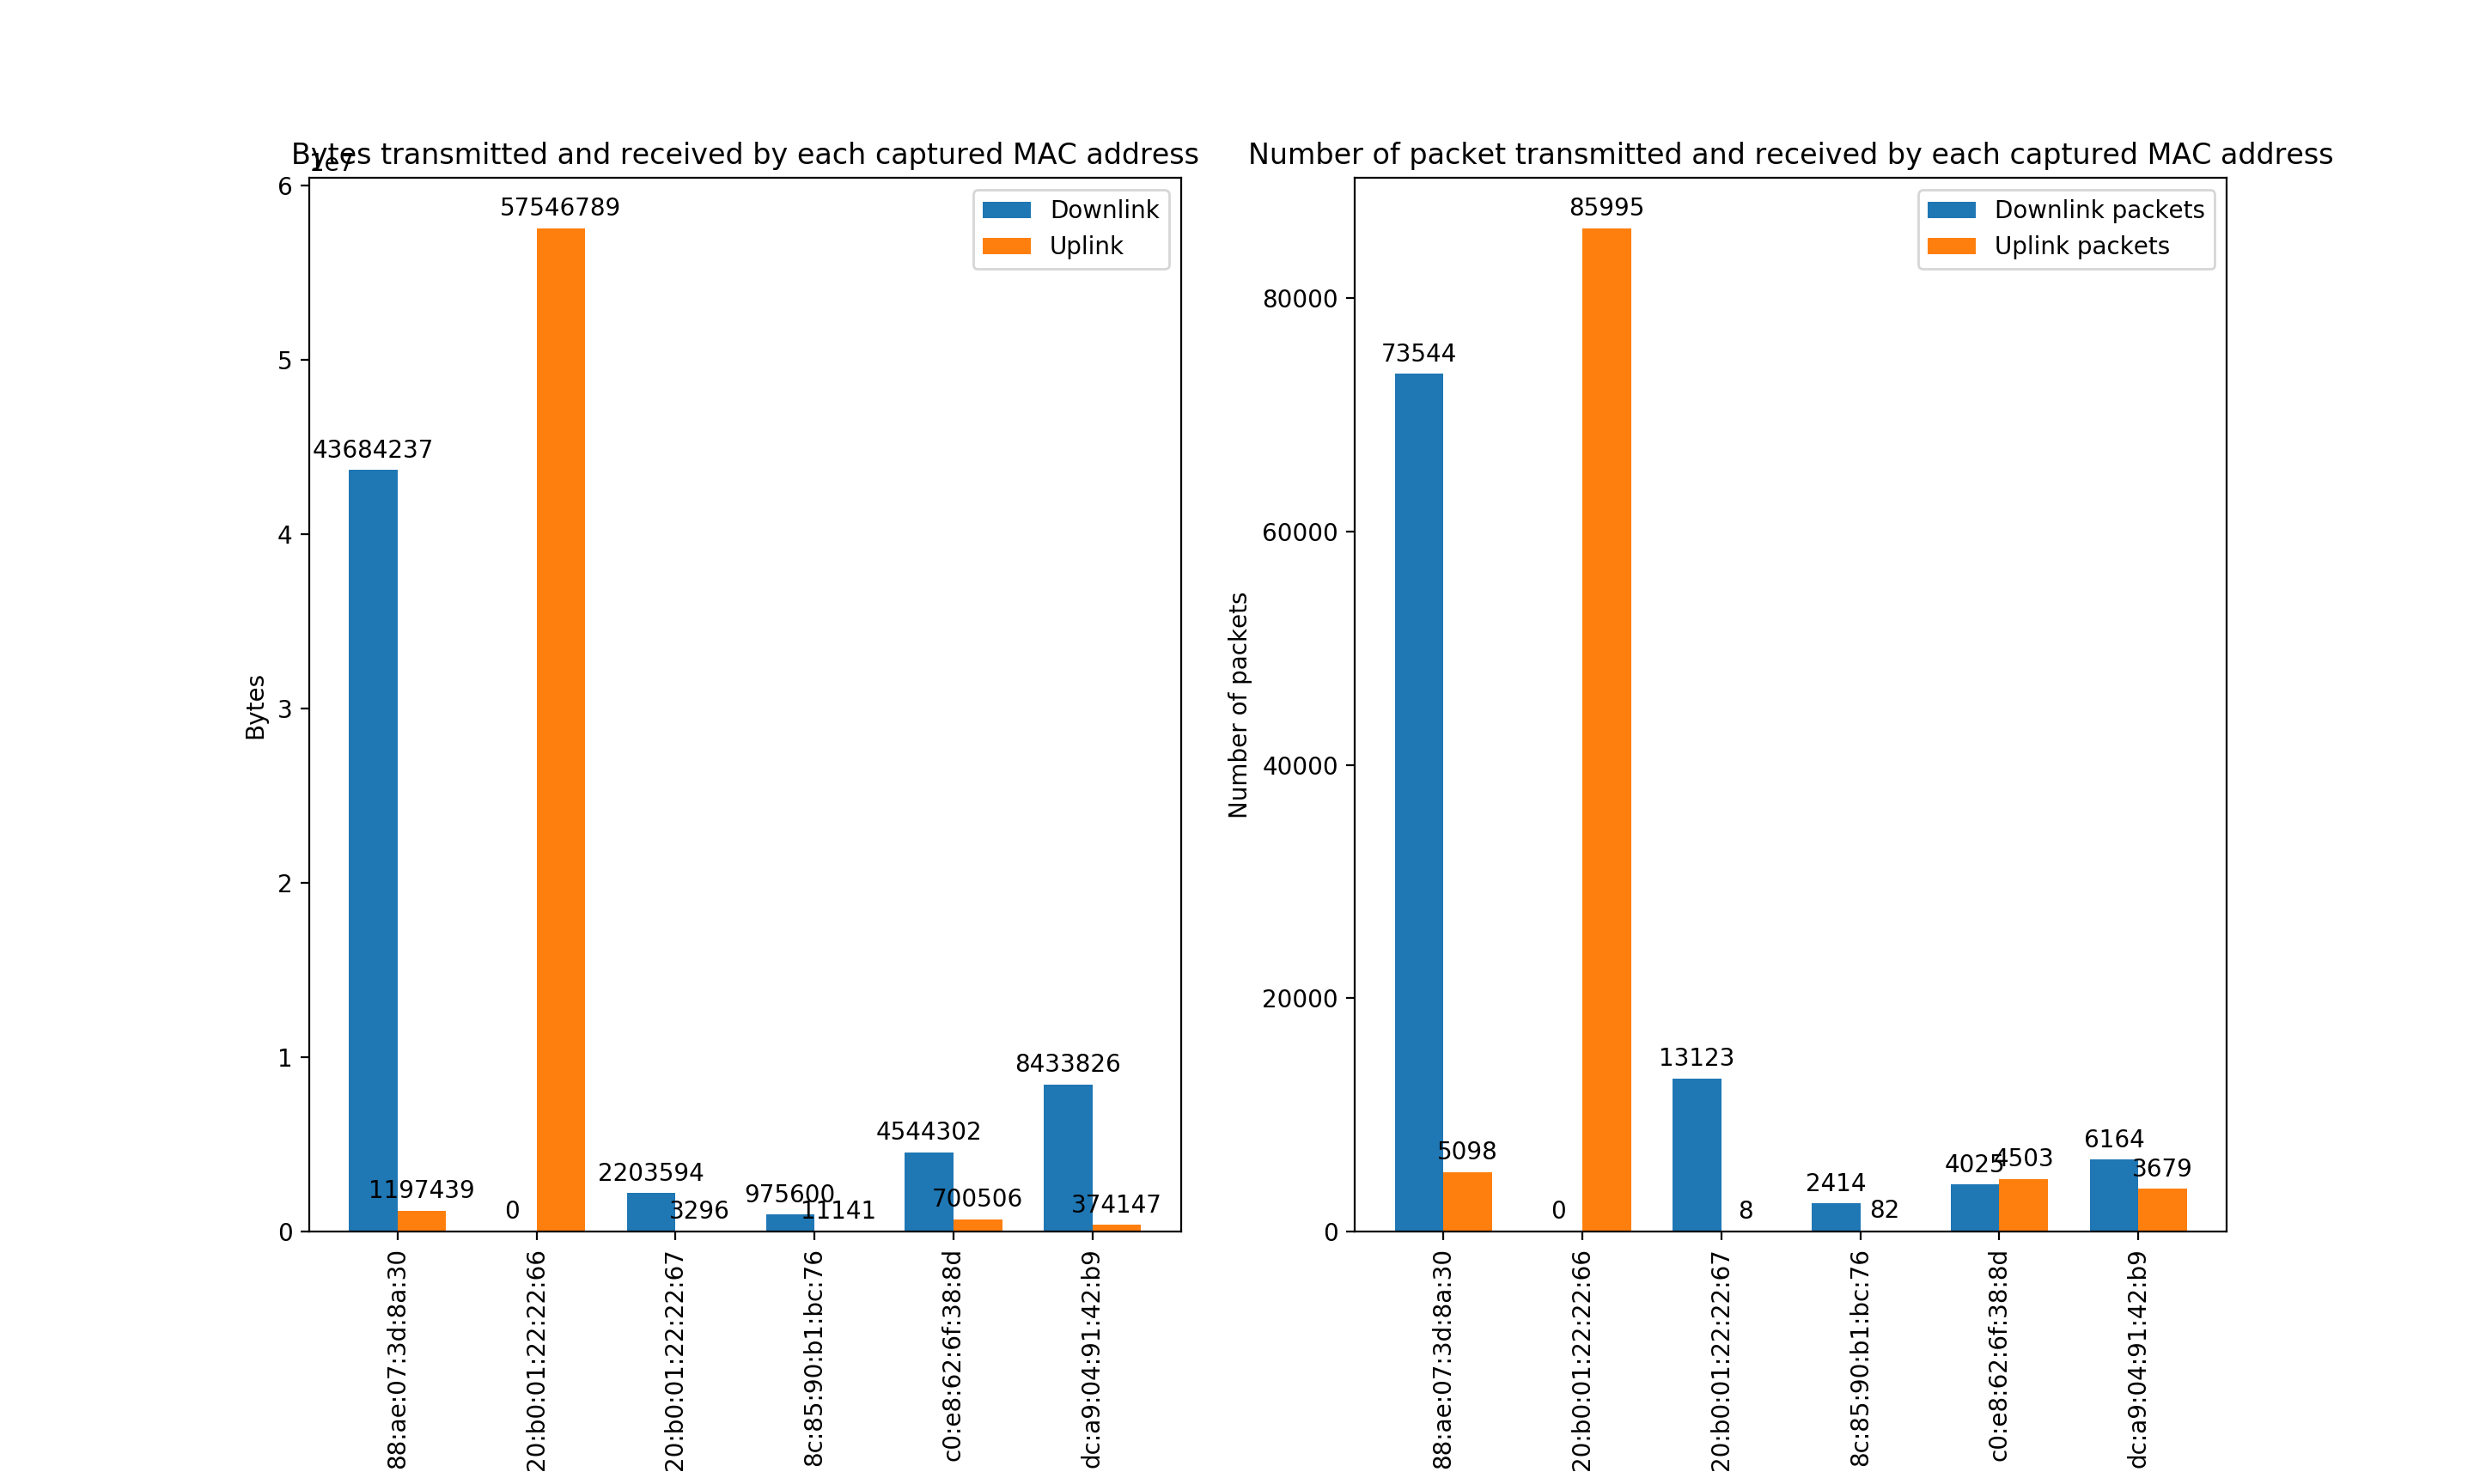
\includegraphics[width=\linewidth]{/Users/lucaferraro/Desktop/PoliMi/First_year/Wireless_networks/Wirelesss_internet/Wireless_internet_project/Graphs/Multimedia_internet_bytes_packets.png}
    \caption{Multimedia internet lecture: data and packets exchanged.}
    \label{fig:Multimedia internet lecture: data and packets exchanged.}
\end{figure}




\subsection{Launch time capture.}
%Luca



\end{document}